%% LaTeX Beamer presentation template (requires beamer package)
%% see http://latex-beamer.sourceforge.net/
%% idea contributed by H. Turgut Uyar
%% template based on a template by Till Tantau
%% this template is still evolving - it might differ in future releases!

\documentclass[hyperref={pdfpagelabels=false}]{beamer}

\mode<presentation>

\usepackage{graphicx}
\usetheme{isu}
\usepackage{times}
\usepackage{amsmath,amsthm, amssymb, latexsym}
\boldmath
\usepackage[english]{babel}
\usepackage[latin1]{inputenc}

\DeclareGraphicsExtensions{.pdf,.jpg,.png}
\graphicspath{{figures/}}

\title[Proposal]{
    A Tale of Two Language Models:\linebreak
    Formally Validating Pig Compilation Algorithm
}
\author[Team Axum: David Johnston and Bijon Bose]{Team Axum: David Johnston and Bijon Bose}
\institute[ISU]{
    Department of Computer Science \linebreak
    Iowa State University\linebreak
    dwtj@iastate.edu\linebreak
    bkbose@iastate.edu
}

\date[COMS 641]{COMS 641: Data Intensive Languages and Systems - Design and Semantics}
%\date{Month X, 20XX}


% If you have a file called "university-logo-filename.xxx", where xxx
% is a graphic format that can be processed by latex or pdflatex,
% resp., then you can add a logo as follows:

%\pgfdeclareimage[height=0.25cm]{logo}{figures/logo}
%\logo{\pgfuseimage{logo}}


\begin{document}
  \begin{frame}[plain]
    \titlepage
  \end{frame}

  \section*{Overview}

\begin{frame}
\begin{itemize}
  \item The Problem
  \begin{itemize}
    \item % TODO What is the problem we solved
  \end{itemize}

  \item Our Approach
  \begin{itemize}
    \item % TODO What is our proposed solution to the problem
  \end{itemize}

  \item Evaluation
  \begin{itemize}
    \item % TODO Perhaps overview the evaluation
  \end{itemize}

  \item Benefits
  \begin{itemize}
    \item % TODO What are the benefits of our solution
  \end{itemize}
\end{itemize}
\end{frame}

  \section{The Problem}
\begin{frame}
  \frametitle{Course Rationale: Prevent This Class of Errors}
  \begin{quote}
      Language and framework-specific errors, i.e. errors that arise due to
      incorrect understanding of the semantics of the language and/or framework
      and its guarantees.
  \end{quote}
\end{frame}

\begin{frame}
  \frametitle{Program Correctness From Compilation Correctness}
  \begin{enumerate}
    \item Programs written in Pig are compiled to MapReduce programs.
    \item A Pig program's correctness requires correct compilation.
    \item Correct compilation depends upon a non-trivial mapping from
      properties over Pig semantics to properties over MapReduce semantics.
  \end{enumerate}

\end{frame}

\subsection{Background}
\begin{frame}{Pig Latin Compilation}
\begin{itemize}
	\item Parser verifies the programs, performs type checking, schema inference and other tasks.
	\item It outputs a canonical logical plan.
	\item The logical plan is optimized and compiled to a series of Map-Reduce Jobs.
	\item The DAG of optimized Map-Reduce jobs are sorted topologically and jobs are submitted to Hadoop for execution. 
\end{itemize}
\end{frame}

\subsection{MapReduce}
\begin{frame}{Execution Model}
\begin{itemize}
	\item Map: Produces a stream of data items annotated with keys.
	\item Local Sort: Orders the data at each machine by key.
	\item Combiner: Performs partial aggregation on the locally ordered data.
	\item Shuffle: Redistributes the data to achieve global ordering.
	\item Merge/Combine: All data received at a particular machine is combined to into a single stream in merge stage.
	\item Reduce: Finally the reduce stage processes the data associated with each key and performs aggregation of the output results.
\end{itemize}
\end{frame}

\begin{frame}{MapReduce Execution Model}
\centerline{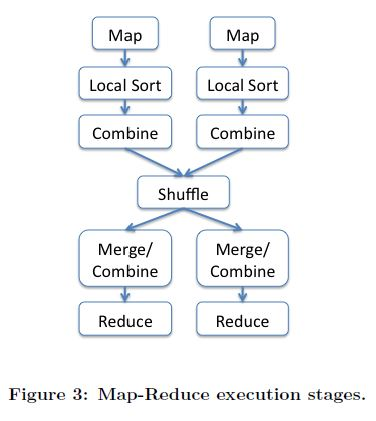
\includegraphics[scale=0.5]{Images/MapReduce_Execution.JPG}}
\let\thefootnote\relax\footnotetext{\tiny The Pig Experience - Gates et al.} 
\end{frame}

\subsection{Pig Latin Compilation}
\begin{frame}{Logical Plan Structure}
\begin{itemize}
	\item A Pig Latin program is a sequence of steps, each of which carries out a single transformation.
	\item Each Pig Latin program is translated to a logical plan
	\item Pig then translates the logical plan to a physical plan and embeds each physical operator inside a Map-Reduce stage to arrive at the Map-Reduce plan.
\end{itemize}
\end{frame}

\begin{frame}{PigLatin - Logical Plan}
\centerline{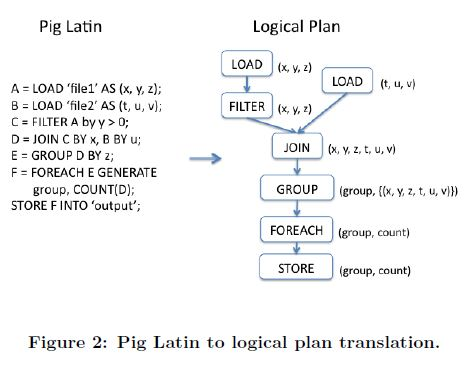
\includegraphics[scale=0.55]{Images/PigLatin.JPG}}
\let\thefootnote\relax\footnotetext{\tiny The Pig Experience - Gates et al.}
\end{frame}

\subsection{Generating MapReduce Jobs}
\begin{frame}{Logical-MapReduce}
\begin{itemize}
	\item Pig translates the logical plan to a physical plan
	\item Logical (CO)GROUP operator translates to - local rearrange, global rearrange and package.
	\item The JOIN is handled either with a COGROUP followed by a FOREACH or fragment replicate join.
	\item After the physical plan is generated Pig assigns physical operators to Hadoop Stages
\end{itemize}
\end{frame}

\begin{frame}
\centerline{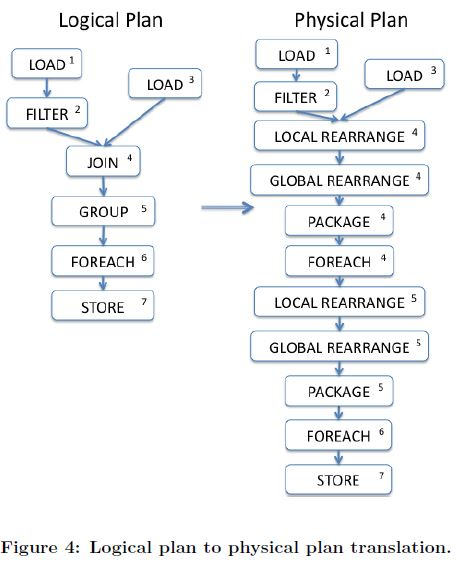
\includegraphics[scale=0.45]{Images/Logical_Physical.JPG} }
\let\thefootnote\relax\footnotetext{\tiny The Pig Experience - Gates et al.}
\end{frame}

\begin{frame}
\centerline{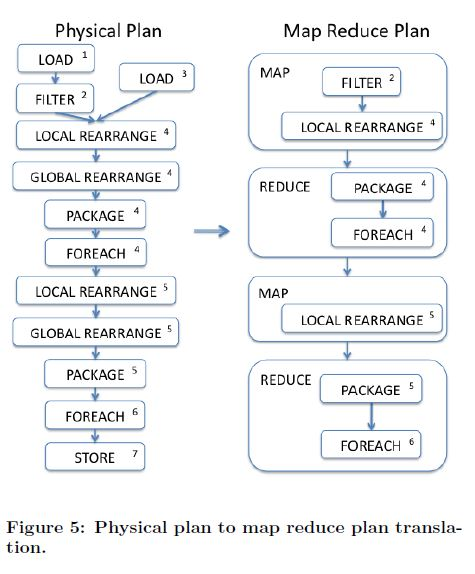
\includegraphics[scale=0.45]{Images/Physical_MapReduce.JPG}}
\let\thefootnote\relax\footnotetext{\tiny The Pig Experience - Gates et al.}
\end{frame}

\begin{frame}
\begin{itemize}
	\item Pig compiles programs written in Pig Latin
	\item Ultimately translates to Map-Reduce tasks
	\item Pig also operates on local mode running on a single machine without map-reduce
	\item There lies an equivalence between PigLatin and MapReduce operational semantics
	\item The equivalence needs to be formalized and correctness needs to be proved  
\end{itemize}
\end{frame}
  \section{Our Approach}

\begin{frame}
\begin{itemize}
  \frametitle{Stages of Project Development}

  \item Identify program equivalency (correctness) properties:
  \begin{itemize}
    \item Initially just functional equivalence?
  \end{itemize}

  \item Identify Pig programs over which we will write proofs:
  \begin{itemize}
    \item Programs with limited data types?
    \item Programs without user defined functions (UDFs)?
    \item Programs with some subset of UDFs?
    \item All well-typed programs?
  \end{itemize}

  \item Implement all of this in Coq:
  \begin{itemize}
    \item Two languages.
    \item Two semantic models.
    \item Existing compilation algo.
    \item Prove correctness/equivalency w.r.t. this compilation algo.
  \end{itemize}

\end{itemize}
\end{frame}

\begin{frame}
  \frametitle{Concurrency in Operational Semantics}
  We expect that Pig should be able to modeled with sequential or non-concurrent
  semantics.

  However, MapReduce should be modeled with concurrent semantics.
\end{frame}

\begin{frame}
  \frametitle{Concern}
  Our correctness proofs should be performed over all (admissible) concurrent
  executions and w.r.t. a parameterized number of mappers and reducers.
\end{frame}

\begin{frame}
  \frametitle{Nondeterministic MapReduce Operational Semantics}
  \begin{figure}
    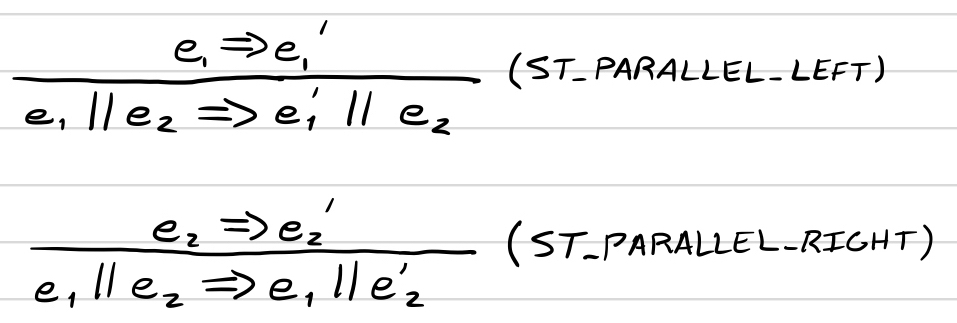
\includegraphics[scale=0.33]{img/ST_PARALLEL.jpeg}
    \caption{Nondeterminism of two MapReduce reduction rules should enable
             semantics to model the uncertain ordering by which concurrent tasks
             are performed.}
  \end{figure}
\end{frame}

\begin{frame}
  \frametitle{Nondeterministic MapReduce Operational Semantics}
  \begin{figure}
    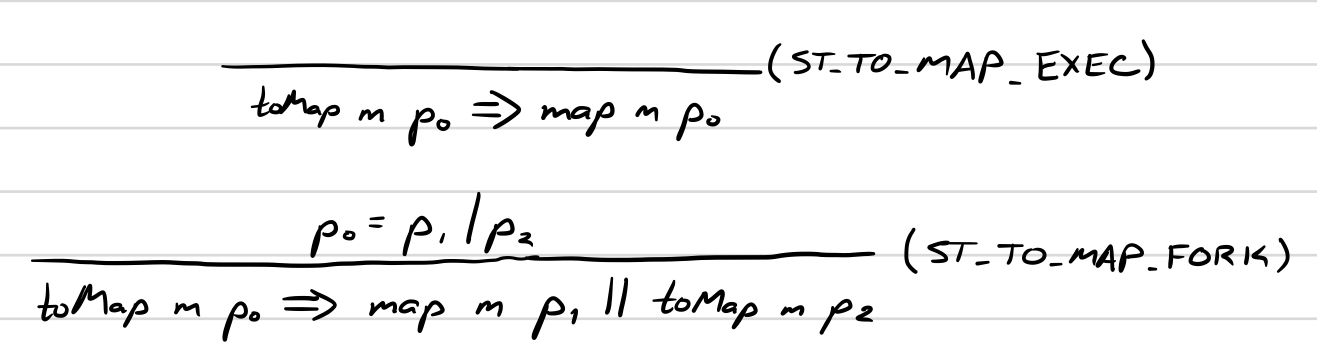
\includegraphics[scale=0.25]{img/ST_TO_MAP.jpeg}
    \caption{Nondeterminism of two MapReduce reduction rules should enable
             semantics to model any number of map task partitions, where each
             task may be given \emph{any} partition of the data.}
  \end{figure}
\end{frame}

  %\section{Evaluation}

\begin{frame}{Evaluation}
To evaluate the formalization technique we aim to use -
\begin{itemize}
	\item Correctness proofs of the model using Coq, constructed with the help of functions and lemmas related to the properties of the functions.
	\item Applying our formalization to actual MapReduce applications like wordcount problem.
\end{itemize}
\end{frame}

  \section*{Summary}

\begin{frame}{Related Work}
  \begin{itemize}
    \item Pig Latin: A Not-So-Foreign Language for Data Processing - Christopher Olsten, Benjamin Reed, Utkarsh Srivastava, Ravi Kumar, Andrew Tomkins
	\item Building a HighLevel Dataflow System on top of MapReduce:The Pig Experience - Alan F. Gates, Olga Natkovich, Shubham Chopra, Pradeep Kamath, Shravan M. Narayanamurthy, Christopher Olston, Benjamin Reed, Santhosh Srinivasan, Utkarsh Srivastava, Yahoo Inc.
	\item Formal Derivation of Distributed MapReduce - Inna Pereverzeva, Michael Butler, Asieh Salehi Fathabadi, Linas Laibinis1, and Elena Troubitsyna
	\item Google's MapReduce programming model - Ralf Lammel
  \end{itemize}
\end{frame}

\begin{frame}{Related Work}
  \begin{itemize}
    \item Using Coq in Specification and Program Extraction of Hadoop MapReduce Applications - Ono, K., Hirai, Y., Tanabe, Y., Noda, N., Hagiya, M.
    \item Formalizing MapReduce with CSP - Yang, F., Su, W., Zhu, H., Li, Q.
    \item Map-reduce-merge: Simplified relational data processing on large clusters - H. C. Yang, A. Dasdan, R.L. Hsiao, and D. S. Parker
   	\item MapReduce: Simplified Data Processing on Large Clusters - Dean, J., Ghemawat, S.
  \end{itemize}
\end{frame}


\begin{frame}{Future Work}
  \begin{itemize}
    \item % TODO Talk about future work/limitations here
  \end{itemize}
\end{frame}


\begin{frame}{Conclusion}
% TODO copy/paste overview here (from intro.tex)
\end{frame}


\begin{frame}
\begin{beamercolorbox}[center]{white}
  {\Large Questions?}

  \vspace{2em}\hfill

  \url{http://www.cs.iastate.edu/~WEBSITE/}
\end{beamercolorbox}
\end{frame}


  \appendix

% make sure you have a blank slide in case you accidentally go past your conclusion
\begin{frame}
  % Nothing here.
\end{frame}


% these slides are to help answer potential questions and generally arent shown
% unless needed or there is extra time
\begin{frame}[plain]{Hidden Slide 1}
\end{frame}

\begin{frame}[plain]{Hidden Slide 2}
\end{frame}

\end{document}
